\documentclass[11pt]{article}
\usepackage[a4paper,margin=2.2cm]{geometry}
\usepackage{amsmath,amssymb,booktabs,graphicx,xcolor,array}
\usepackage[colorlinks=true,linkcolor=blue!50!black]{hyperref}
\definecolor{freeblue}{RGB}{21,101,192}
\newcommand{\free}[1]{{\color{freeblue}#1}}
\setlength{\parindent}{0pt}\setlength{\parskip}{6pt}

\title{The linear power spectrum of the model-independent analysis\\[2pt]
\large what is fixed, what is free (DESI DR1 FS+BAO, model \texttt{Ag245F})}
\date{4 October 2026}
\begin{document}
\maketitle

\section{The model}

\begin{equation}
\boxed{\;
P_{\rm lin}(k,z_i)\;=\;
\underbrace{\free{\left[\frac{D(z_i)}{D(z_N)}\right]^{2}}}_{\text{growth}}\;
\underbrace{\free{a(k)}}_{\text{broadband}}\;
\underbrace{T_{\rm nw}(k)}_{\substack{\text{smooth}\\ \text{fiducial}}}\;
\Bigg[\,1+\underbrace{\big(1+\free{A}\big)}_{\substack{\text{BAO}\\ \text{amplitude}}}\;
\underbrace{e^{-k^2\free{\Delta\Sigma^2}/2}}_{\text{damping}}\;
\underbrace{O\big(\free{\alpha_{r_s}}\,k\big)}_{\substack{\text{fiducial wiggles,}\\ \text{rescaled by } r_s}}\Bigg]
\;}
\label{eq:pklin}
\end{equation}

\textbf{\free{Blue} = free, sampled. Black = fixed}, computed once from the fiducial cosmology and never changed.

\textbf{Check.} At the fiducial values $a\equiv1$, $A=0$, $\Delta\Sigma^2=0$, $\alpha_{r_s}=1$ and $z_i=z_N$,
eq.~\eqref{eq:pklin} gives $P_{\rm lin}(k,z_N)=T_{\rm nw}(k)\,[1+O(k)]=T(k)$, the fiducial spectrum, exactly.

\textbf{Redshifts.} The spectrum is reconstructed at a single redshift, $z_N=1.491$ (QSO), the farthest of the six.
At the other sample redshifts, $z_i\in\{0.295,\,0.510,\,0.706,\,0.919,\,1.317\}$, it has the same shape and only the
amplitude changes, through $D(z_i)/D(z_N)$.

\section{The fixed part: the fiducial model}

\begin{itemize}\itemsep2pt
\item \textbf{Fiducial cosmology} (the DESI fiducial, Planck 2018): flat $\Lambda$CDM with $\omega_b=0.02237$,
  $\omega_{\rm cdm}=0.1200$, $h=0.6736$, $\ln(10^{10}A_s)=3.044$, $n_s=0.9649$.
\item $T(k)\equiv P^{\rm fid}_{\rm lin}(k,z_N)$: its linear spectrum at $z_N$. It is computed with CosmoPower at
  $z=5$ and grown to $z_N$ with $\Lambda$CDM growth.
\item \textbf{The split} $T=T_{\rm nw}\,(1+O)$, done once:
  \begin{itemize}\itemsep1pt
  \item $T_{\rm nw}(k)$ is the smooth part: the Eisenstein--Hu no-wiggle shape times the ratio $T/T_{\rm EH}$ smoothed
    with a Gaussian of 0.25 dex in $k$.
  \item $O(k)=T/T_{\rm nw}-1$ is the BAO wiggle pattern. It is at most $6.6\%$, its largest peak is at
    $k=0.050\,{\rm Mpc}^{-1}$, and it is set to zero below $3\times10^{-3}\,{\rm Mpc}^{-1}$.
  \end{itemize}
\item $k$ is in ${\rm Mpc}^{-1}$, converted with the fiducial $h$.
\end{itemize}

\begin{figure}[h]
\centering
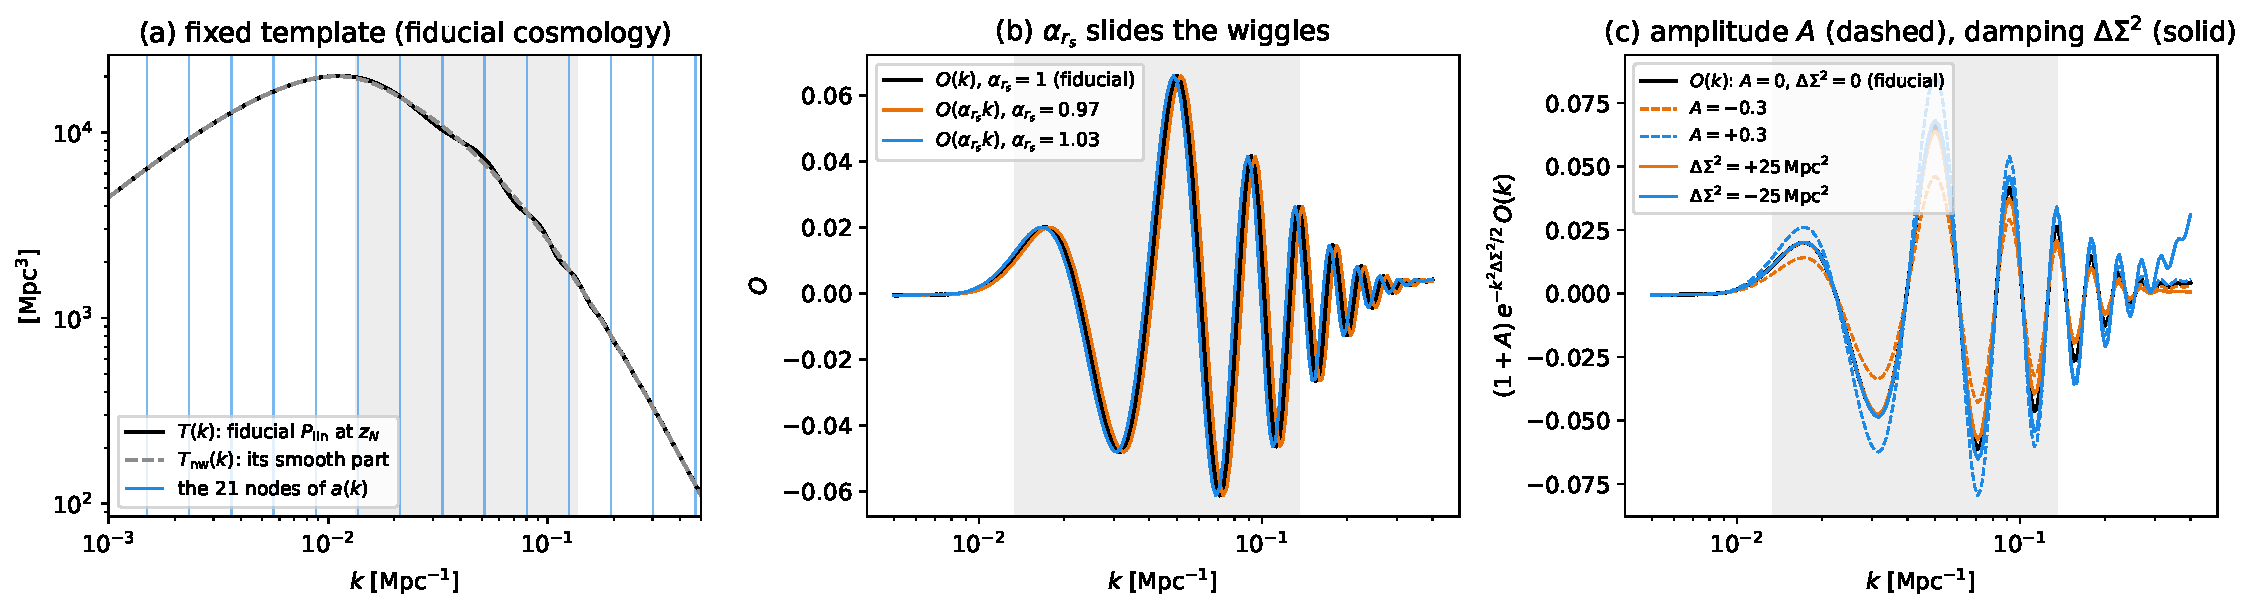
\includegraphics[width=\textwidth]{pklin_template.pdf}
\caption{(a) The fixed template $T$, its smooth part $T_{\rm nw}$, and the 21 nodes of $a(k)$; the grey band is the
data range, $0.02$--$0.2\,h/{\rm Mpc}$. (b) $\alpha_{r_s}$ slides the wiggles. (c) $A$ scales them at every $k$
(dashed); $\Delta\Sigma^2$ damps them, or undamps them when negative, more strongly at high $k$ (solid).}
\end{figure}

\section{The free parameters}

\renewcommand{\arraystretch}{1.25}
\begin{tabular}{@{}>{\color{freeblue}}l c p{6.4cm} p{4.2cm}@{}}
\toprule
\color{black}parameter & \color{black}number & \color{black}what it does & \color{black}prior \\
\midrule
$D(z_i)/D(z_N)$ & 5 & Amplitude at sample redshift $z_i$ relative to $z_N$ (it is 1 at $z_N$). &
  amplitude at each $z_i$: $\pm0.6$ in $\ln P$ \\
$a(k)$ & 21 & Broadband shape and the overall amplitude at $z_N$.
  $a=\exp[\text{cubic spline of }\ln a_j\text{ in }\ln k]$, with nodes uniform in $\ln k$ over
  $10^{-4}$--$0.7\,h/{\rm Mpc}$ (spacing 0.443), constant outside. &
  shape: $\pm0.5$ per node, plus smoothness; mean of $\ln a_j$: amplitude prior \\
$\alpha_{r_s}$ & 1 & Rescales the wiggles by the sound horizon: a peak at $k_p$ moves to $k_p/\alpha_{r_s}$. In a cosmology,
  $\alpha_{r_s}=(h\,r_d)/(h\,r_d)_{\rm fid}$. & $\ln\alpha_{r_s}\sim\mathcal N(0,0.05)$ \\
$A$ & 1 & BAO amplitude: the wiggles are multiplied by $(1+A)$ at every $k$. & $\mathcal N(0,0.3)$ \\
$\Delta\Sigma^2$ & 1 & Damping of the linear wiggles relative to the fiducial, $e^{-k^2\Delta\Sigma^2/2}$; negative means less damped. & $\mathcal N(0,25\,{\rm Mpc}^2)$ \\
\midrule
\color{black}total in $P_{\rm lin}$ & \color{black}29 & & \\
\bottomrule
\end{tabular}

\smallskip
\textbf{Priors in detail.}
\begin{itemize}\itemsep1pt
\item The shape prior acts on $\ln a_j-\langle\ln a\rangle$. It is $\sigma=0.5$ per node plus
  $\lambda\sum_j(\ln a_{j+1}-2\ln a_j+\ln a_{j-1})^2$, with $\lambda=7.78$.
\item The amplitudes $u_i=\langle\ln a\rangle+2\ln[D(z_i)/D(z_N)]$, with $u_N=\langle\ln a\rangle$, are Gaussian
  with covariance $(0.5^2/21)\,\mathbf{1}\mathbf{1}^{\sf T}+0.6^2\,\mathbb{1}$.
\item All priors are centred on the fiducial.
\end{itemize}

\section{Relation to a standard BAO template}

A Fourier-space BAO fit models the observed spectrum as $P_{\rm nw}(k)\,[1+O(k')\,e^{-k^2\Sigma^2/2}]$, plus a free
broadband. $k'$ is $k$ dilated by $\alpha=(D/r_d)/(D/r_d)_{\rm fid}$. Eq.~\eqref{eq:pklin} has the same structure: a
fixed fiducial wiggle pattern, rescaled only through the sound horizon, with a free amplitude and damping. It differs in
three places.
\begin{enumerate}\itemsep2pt
\item \textbf{It is the \emph{linear} spectrum.} It goes through the one-loop EFT, so the nonlinear BAO damping comes from
  pybird's IR resummation. $\Delta\Sigma^2$ is only the change of the \emph{linear} (Silk) damping from the fiducial, which
  depends on $\omega_b/\omega_m$. It is small and can be negative.
\item \textbf{The broadband multiplies the wiggles.} $a(k)$ is free but too coarse (21 nodes) to follow or slide a wiggle,
  so it carries no BAO information. Because it multiplies the wiggles too, it cannot change their size relative to the
  smooth part; a BAO fit gets that freedom from its additive broadband terms. $A$ provides it here. Without $A$ (damping
  alone) real spectra cannot be represented.
\item \textbf{The BAO dilation is split in two.} $\alpha_{r_s}$ rescales the wiggles; the per-redshift AP dilations
  $\alpha_\parallel(z_i)$ and $\alpha_\perp(z_i)$ dilate the whole spectrum, wiggles and broadband alike. The BAO points
  depend only on the combination $\alpha/\alpha_{r_s}=(D/r_d)/(D/r_d)_{\rm fid}$, as in a BAO fit. $\alpha_{r_s}$ itself is
  close to prior-limited.
\end{enumerate}

\textbf{Not part of $P_{\rm lin}$:} the growth rate $f(z_i)$ and the AP dilations $\alpha_\parallel(z_i)$ and
$\alpha_\perp(z_i)$ enter afterwards, in pybird's redshift-space and AP mapping.

\end{document}
